%------------------------------------------------------------------------------
% This is a LaTeX template for the scientific justification of IRAM Proposals
%------------------------------------------------------------------------------
%
% You may customize this template to suit your preferences (e.g. using BibTex),
% but please respect the following requirements:
%     The scientific and technical justification should contain a
%     maximum of 2 pages of text (4 pages for Large Programs),
%     plus 2 pages of Figs., Tables and Refs.
%     Don't mix text with figures, tables, and references !!
%     The font size should be 11pt or larger.
%
%------------------------------------------------------------------------------
%
\documentclass[11pt,a4paper,twoside,graphicx,color]{article}
%
\usepackage[margin=2cm]{geometry}
\usepackage{graphics,graphicx}
\usepackage[update,prepend]{epstopdf}
\usepackage[innercaption]{sidecap}
\usepackage{subcaption}
\usepackage{amssymb, amsmath}
\usepackage{xspace}
\usepackage{natbibspacing, natbib}
\usepackage{aas_macros}
\usepackage{wrapfig}
\usepackage{floatrow}

\newcommand{\ncrit}{\mbox{$n_{\rm crit}$}\xspace}
\newcommand{\comol}{$^{12}$CO\xspace}
\newcommand{\Lsun}{\mbox{$L_{\odot}$}\xspace}
\newcommand{\LIR}{\mbox{$L_{\rm IR}$}\xspace}
\newcommand{\LFIR}{\mbox{$L_{\rm FIR}$}\xspace}
\newcommand{\Msun}{\mbox{$M_{\odot}$}\xspace}
\newcommand{\mstar}{\mbox{$M^*$}\xspace}
\newcommand{\sfrsd}{\mbox{$\Sigma_{\rm SFR}$}\xspace}
\newcommand{\sfrU}{\mbox{\Msun\,yr$^{-1}$}\xspace}
\newcommand{\rarr}{$\rightarrow$}
\newcommand{\vs}{$v_{\rm rot}/\sigma$\xspace}
\newcommand{\aco}{\mbox{CO(1-0)}\xspace}
\newcommand{\bco}{\mbox{CO(2-1)}\xspace}
\newcommand{\cco}{\mbox{CO(3-2)}\xspace}
\newcommand{\dco}{\mbox{CO($J$=4$-$3)}\xspace}
\newcommand{\eco}{\mbox{CO($J$=5$-$4)}\xspace}
\newcommand{\fco}{\mbox{CO($J$=6$-$5)}\xspace}
\newcommand{\gco}{\mbox{CO($J$=7$-$6)}\xspace}
\newcommand{\rot}[3][HCN]{\mbox{#1($J$=#2\rarr#3)}\xspace}
% default HCN; usage \rot[HCN]{3}{2} or \rot[\hcop]{4}{3}
\newcommand{\Lp}[1][CO]{\mbox{$L^{\prime}_\textrm{\fontsize{8pt}{12pt}\selectfo
nt{#1}}$}}
\newcommand{\LpU}{\mbox{K\,\,km\,\,s$^{-1}$\,\,pc$^2$}}
\newcommand{\kms}{km\,s$^{-1}$\xspace}
\newcommand{\pmOne}{\mbox{$^{-1}$}\xspace}
\newcommand{\Fig}[1]{Fig.~\ref{fig:#1}}
\newcommand{\Eq}[1]{Equation~\ref{eq:#1}}
\newcommand{\E}[1]{\mbox{$\times10^{#1}$}}
\newcommand{\eq}{\,=\,}
\newcommand{\ssim}{\,$\sim$\,}
\newcommand{\pmm}{\,$\pm$\,}
\newcommand{\ncode}[1]{{\sc #1}}
\newcommand{\uvmcmcfit}{\ncode{uvmcmcfit}\xspace}

\newcommand{\mulw}{multi-wavelength\xspace}
\newcommand{\SF}{star formation\xspace}
\newcommand{\galpop}{galaxy populations\xspace}
\newcommand{\SB}{starburst\xspace}
\newcommand{\SBs}{starbursts\xspace}
\newcommand{\highz}{high-$z$\xspace}
\newcommand{\athighz}{at high redshift\xspace}
\newcommand{\interz}{intermediate-$z$\xspace}
\newcommand{\atinterz}{at intermediate redshift\xspace}
\newcommand{\obs}{observations\xspace}
\newcommand{\gl}{gravitationally lensed\xspace}
\newcommand{\qh}{quasar host galaxy\xspace}
%%%%%%%%% Compact BIB %%%%%%%%%%
\citestyle{aa}
\bibliographystyle{apj_w_etal_3auth}

\usepackage{paralist}

\renewenvironment{thebibliography}[1]{%
%\section*{\refname}%
%  {\normalsize {\textbf{References:}}}
  \let\par\relax\let\newblock\relax%
  \inparaitem[{[}1{]}]}{\endinparaitem}
%%%%%%%%%%%%%%%%%%%%%%%%%%%%%


%
% Page size and text dimensions
% Do not change!
\textheight 260mm
\textwidth 178mm
\oddsidemargin -8mm
\evensidemargin -8mm
\marginparwidth 50pt
\topmargin -22mm
\brokenpenalty=10000
\sloppy
%
%-------------------------------------------------------------------
\begin{document}
%
%
\begin{center}{\LARGE \bf
%-------------------------------------------------------------------
2-kpc resolution \cco imaging of an exceptional strongly-lensed wet-merger at $z$$\sim$0.65
%-------------------------------------------------------------------
}\end{center}
\centerline{\bf P.I.: T. K. Daisy Leung}
\vspace{0.5em}
\noindent {\bf Star formation modes and molecular gas dynamics beyond the local universe} \\
\indent Tremendous progress has been made towards our understanding of the \highz
universe over the past two decades \citep[see recent reviews by][]{CW13,Madau14a, Casey14a}. These studies
suggest that the elevated \SF rates (SFRs) and specific SFRs observed in galaxies at
the peak epoch of \SF (1$\lesssim$$z$$\lesssim$3) are
primarily driven by their increased in molecular gas mass fractions and \SF efficiencies (SFEs) compared to
local galaxies, and that \SF in these early systems can be grossly categorised into
two dominant modes -- a quiescent mode in disk-like galaxies versus a starburst mode in commonly merger-driven
 \SB and quasar host galaxies \citep[e.g.][]{Sargent12a}.
% brings up the spatial resolution
The systematically enhanced molecular gas fractions observed in \highz
\galpop imply that their star-forming clumps are expected to be larger in size due to
larger internal turbulence
compared to nearby galaxies.  % Elmegreen & Elmegreen 2005, Bournaud+08
Indeed, recent studies have found gas clumps on the order of
$\sim$1$-$2\,kpc scales at $z$\ssim1--2 \citep[e.g.][]{Genzel11a, Swinbank12a, Swinbank12b},
% and R_{\rm 1/2} $\sim$5\,kpc disks form $\sim$1\,kpc clumps \citep{Genzel11a},
providing direct evidence that the
interstellar medium (ISM) conditions of galaxies evolve as a function of cosmic time. This
highlights the importance of resolving gas dynamics of galaxies on these scales
and at earlier epochs in order to investigate the
mechanisms and physical processes responsible for % leading to
the two \SF modes and for causing the steep decline in the cosmic SFR density since $z$\ssim1.5 \citep[e.g.][]{Lagos11a,Popping12a}.

% how it's been proposed to connect to local
While studies using spatially resolved CO \obs in
local ultra-luminous IR galaxies (ULIRGs) and their \highz analogues ($z$$\gtrsim$1 \SB systems)
have enabled a better understanding of the gas properties of mergers at these epochs
\citep[e.g.][]{Carilli10a, Engel10a,Bothwell10a,Riechers11b, Ivison11a},
% kinematic and dynamical evidence that massive \highz \SB galaxies are formed in major mergers
% distinct kinematic components and disturbed gas morphologies
% that are likely the progenitors of local massive ellipticals
the gas excitation, distribution, and dynamics of mergers
\atinterz (0.6\,$\lesssim$\,$z$\,$\lesssim$\,1) --- the epoch where the \SF history is steeply rising --- remain largely unknown
due to the lack of spatially resolved CO observations at these redshifts.
Thus, to understand of the role of mergers throughout cosmic history and
to obtain a coherent picture connecting \highz populations to present-day galaxies,
it is vital to carry out detailed studies of the gas kinematics and dynamics \atinterz.

We have sucessfully imaged \bco line emission
in the strongly-lensed quasar host galaxy
 RXJ\,1131$-$1231 (hereafter RX1131) at $z$\ssim0.65
with the PdBI/NOEMA \citep[\Fig{combine};][]{Leung16b}.
We here propose to image {\bf \cco}
at higher resolution using the {\bf A+C array configurations}.
By combining the magnification provided by gravitational lensing with the excellent spatial resolution and sensitivity of NOEMA,
we will study the internal gas dynamics and distribution
down to the physical scales of \highz star-forming clumps 
at $\sim$0.6'' resolution 
(corresponding to a physical scale of $\sim$1.8\,kpc in the source plane at the target redshift)
{\bf in only 1.5 hours on source}.
Since our target is currently the only source with spatially resolved CO
imaging at intermediate redshift with existing \mulw analysis spanning rest-frame
UV-to-radio, obtaining the proposed \obs will enable, for the first time, a kpc-scale characterisation of the gas, dust, and stellar populations in a quasar host galaxy and merger at intermediate redshift.

\vspace{0.2em}
\noindent {\bf Unique nature of our target RXJ\,1131$-$1231}\\
\indent
RXJ1131 is a quadruply-imaged optical quasar (bright knots in \Fig{combine}d)
with its host galaxy being lensed
into a partial Einstein ring (\Fig{combine}d \& \Fig{velo}; \citealt{Sluse03a}).
% HST observations (rest-frame UV) have revealed distinct emission
% from recent star-formation (lensing arcs) and from the AGN (bright knots) in the background galaxy,
A source-plane reconstruction
of optical imaging data indicates that the host galaxy displays a disk-like morphology, with
a companion galaxy located at $\sim$2.4 kpc away
\citep[\Fig{combine}f;][]{Claeskens06a, Brewer08a}.
We have recently confirmed that both galaxies are at the same redshift by detecting their
\bco emission and decomposing their gas distribution
via $uv$-plane lens modeling
of the NOEMA \bco data
 in velocity-space \citep[\Fig{combine}c \& e;][]{Leung16b}, finding a gas mass of
$M_{\rm gas}$\ssim1.4\E{10}\,\Msun for RXJ1131.
Our dynamical lens modelling
shows that the asymmetry in the double-horned line profile (\Fig{combine}a)
is mainly a result of differential lensing, where
the magnification factor varies from $\sim$3 to $\sim$9 across
different kinematic components.
The intrinsically symmetric double-horned line
profile of RXJ1131 (\Fig{combine}c) together with its source-plane velocity gradient
and rotation profile (\Fig{velo})
suggest that RX1131 is an extended disk of $\gtrsim$6\,kpc in radius.
% and dynamical mass of $M_{\rm dyn}$\ssim8\E{10}\,\Msun.
% SED
We find a lensing-corrected IR luminosity of 1.5\E{12}\,\Lsun based
on our spectral energy distribution (SED) modelling (\Fig{SED}),
indicating that RXJ1131 is a ULIRG with a SFR\ssim120\,\sfrU.
%Fitting dust SED models to the IR-to-mm photometry, we derive
%a lensing-corrected dust mass of $M_{\rm dust}$\ssim4\E{8}\,\Msun,
%an infrared luminosity of \LIR$\sim$\,1.5\E{12}\,$(5.5/\mu_{\rm L})$\,\Lsun,
%and a far-IR luminosity that corresponds to a SFR$_{\rm FIR}$\ssim120\,\sfrU.
We also find that
RXJ1131 contains
% a gas mass fraction $f_{\rm gas}$\eq$M_{\rm gas}$/$M_{\rm dyn}$\ssim19\%
a baryonic gas fraction of $f_{\rm mol}$\ssim32\%
that is higher than local galaxies but modest compared to $z$\ssim2 disk galaxies \citep{Daddi10a}.

% what have we learned from our data
Despite similar IR luminosity, CO linewidth and SFR found between RXJ1131
and other ULIRGs/high-$z$ \SB galaxies,
its CO source size, gas depletion timescale and SFE are similar to those
of nearby and high-$z$ disk galaxies rather than \SB systems. This suggests that
the \SF in RXJ1131
% is enhanced by % SFR is higher than local disks, similar to highz turbulent disks, but lower than highz SBs
mainly driven by
global gravitational instabilities due to its high gas fraction
rather than merger-induced gas accumulation,
in contrast to local ULIRGs/mergers and \highz starbursts.
On the other hand, we find disturbed gas morphologies with velocity dispersion exceeding
400\,\kms near the central region of RXJ1131 (\Fig{combine}e), but since
the emission is only resolved over $\sim$2$-$3 beams at the resolution of our current data ($\sim$4.4''$\times$2''),
% it is unclear whether the observed dispersion
it is impossible to quantify dispersions due to
perturbations from its AGN,
turbulence from interactions with its companion,
and gravitational instability due to the huge gas reservoir. % owing to beam smearing effect
% Resolving the gas kinematics and dynamics at higher resolution is needed to examine
% the true nature of these observed phenomena and ISM properties. % disk-like SFE, extended disk, but high dispersion

\vspace{0.2em}
\noindent {\bf This proposal} \\
\indent
We propose to map \cco line emission in RXJ1131
which we have already detected with CARMA at moderate S/N and resolution ($\sim$3''; Leung et al. 2016).
Based on scaling relations
% for the Toomre scale length
\citep{Genzel11a}, % , L\_toomre ~ f\_gas *R\_disk, then
we expect clump sizes of % 0.32*6
$\sim$1.9\,kpc in RXJ1131. % given its gas fraction and disk size.
Thus, the proposed resolution of $\sim$0.6'' ($\sim$1.8\,kpc in the source plane at $z$\ssim0.65) will enable us to derive \vs
% (a proxy to the Toomre Q parameter)
on this scale length, enabling us to quantify whether RXJ1131 is a rotation- or dispersion-dominated system,
and to examine its internal dynamics by studying the spatial variations in \vs.
Previous studies have shown that resolutions corresponding to $\sim$1.7$-$2\,kpc are sufficient to withstand %tolerate
beam smearing effect to extract rotation velocity and
dispersion even at $z$\ssim2  \citep[e.g.][]{Newman13a, Genzel14a}.
The \vs ratio together with gas size and surface density will enable us to compute the theoretical Jeans length,
which we will then use to determine the dynamical timescales of the star-forming clumps in RXJ1131
to examine its star-forming conditions and mechanisms.
%(e.g. is it merger-driven).
% which important to our understanding of the build up of local massive disk galaxies.
% ... by smooth accretion of gas and/or minor mergers.
% This will allow us to contrast its dynamical properties between mergers and disks galaxies at low and \highz.
%
% say 1st moment map, rotation profile
We will derive the rotation velocity by reconstructing the intrinsic gas distribution and velocity field using
a similar approach as with our NOEMA \bco data (\Fig{velo}), but at much higher precision.
This will enable us to derive reliable estimates on the rotation velocity, inclination angle, and
dynamical mass by fitting disk models.
% place seven constraints on the rotation profile which is yet
 % at [ 6.29772725  3.02618336  2.29008935  0.          2.45365038  3.844054  6.13413293] kpc

%
% physical properties -- excitation
We will measure spatially resolved line ratios % between the \cco and \bco
% emission
within RX1131 to gain insight into its gas excitation conditions.
The molecular gas distribution, kinematics and line ratio variations will provide clues to
the main driver of \SF in RXJ1131 (e.g. if the warmer gas is
concentrated toward the central region of RX1131 like in nearby ULIRGs),
how interactions with the companion influence the molecular gas
in fueling its ongoing \SF and the central quasar,
and how its gas excitation differs from other \galpop at different cosmic epochs.
% but we would need a way to reconstruct the dispersion via lens modeling.
%
%
% spatially-resolved SK
Additionally, based on our SED model, 
we expect to detect continuum emission underlying the \cco line at $\sim$5-10$\sigma$ significance
and the observed image ratios at radio wavelengths.
% the 2\,mm continuum source size estimated from the publicly release ALMA data at BLAH'', % but if I say this, then that means
% we don't really need this additional cont data to do
Hence, the proposed data will also allow us to place constraints on the spatially resolved
``\SF law'' at $z$\ssim0.65.

% --------------
% final word
Given the rare lensing configuration and nature of our target, the proposed observations
present an excellent opportunity to investigate the molecular gas excitation, kinematic and dynamical
state of a distant quasar host galaxy, allowing
% The proposed high resolution and S/N \cco data will allow
us to investigate how physical parameters, e.g. stellar mass, dust temperature, SFR, SFE, and morphology, which have been investigated at both nearby and $z$$\gtrsim$1 galaxies, vary \atinterz depending on the molecular gas
properties. %, providing important constraints for current models of galaxy evolution.

%Mapping the molecular gas in RXJ1131on the scales of its star-forming clumps and
%constraining the velocity structure, rotation velocity and the dispersion on these scales
%will allow us to study the ISM conditions on these scales to
%investigate whether the \SF mode in RXJ1131is predominantly driven its disk-like kinematics and dynamics.
%% probably because it is a disk, and the companion is only minor
%% but this also means that there are different kinds of mergers, and at different epochs, that have different \SF properties.
%and to gain insights into how the \SF processes in disk galaxies have evolved since the peak epoch of \SF.

\vspace{.2em}
\noindent {\bf Technical justification}
% A+C: ~0.66" at 209 GHz
We propose to observe \cco emission in RXJ1131 at $z_{\rm CO}$\eq0.6537 at a
redshifted line frequency of 209.10443\,GHz ($\nu_{\rm rest}$\eq345.79599\,GHz) using the A+C array configurations.
Given the spatial extent the quasar host galaxy ($\sim$3.8'' in diameter),
we request C-array configuration to provide short spacings
to maximize the sensitivity and $uv$ coverage for lens modelling, and to
ensure that diffuse lensed emission on $\gtrsim$0.4'' scale is not resolved out. % just A array
% To maximize the sensitivity and UV coverage of the maps and to ensure that no flux was resolved out at the highest resolution, we combined the extended configuration data with the compact configuration observations.
We estimate the expected source size based on the
most extended kinematic component in our dynamical lens model of the \bco data, which takes into account the asymmetric line emission and spatial extent across different velocity bins (arising due to differential lensing).
We therefore expect the source to be resolved over $\sim$10 beams at the proposed angular resolution of $\sim$0.66''.
We compute the expected \cco line strength based on our
CARMA \cco line flux of $I$\eq35.7\,Jy\,\kms and line FWHM of $\sim$700\,\kms.
To obtain sufficient S/N for dynamical lens modelling over 10 velocity bins,
we require a 10$\sigma$ detection of $\sigma$\eq1.35
\,mJy\,beam\pmOne per 70\,\kms bin,
{\bf requiring only $\sim$2.2 hours on source} (and 3.4 hours including overheads) with 8 antennas.
We note that the requested sensitivity will correspond to S/N$>$10 for channels with spatially less extended emission, which are also found to have lower magnification factors (and thus lower apparent flux density).

\clearpage
% You may include up to two pages of figures, tables, and References.

%\begin{figure}[!tbhp]
%\hspace{-1.75em}
%\vspace{-0.35em}
%\centering
%\floatbox[{\capbeside\thisfloatsetup{capbesideposition={right,center},capbesidewidth=0.46\textwidth}}]{figure}
%[\FBwidth]
%{\hspace{-0.5em}
%\includegraphics[trim= 10 20 15 0, clip, scale=0.23]{Figures/F555W-eps-converted-to}
%\hspace{-2.0em}
%\includegraphics[trim= 10 0 0 5, clip, scale=0.33]{Figures/Manipulate_figsCROP}
%\vspace{-1.0em}
%}
%{
%\hspace{-1.05em}
%\caption{\fontsize{11pt}{12.5pt}\selectfont{\textbf{Stellar light distribution in
%the AGN host galaxy RXJ 1131-1231 and its reconstructed source plane morphology.}
%{\em Left:} Rest-frame UV emission (tracing recent star formation)
%is lensed into an almost complete Einstein ring with diameter $\sim$3.8".
%{\em Right:} Lens modeling of the optical emission identifies complex
%structures in the host galaxy and
%an optically faint companion (white component as indicated by the blue arrows;
%\citealt{Claeskens06a}),
%which we have recently confirmed by lens-modeling our \bco data
%(\Fig{combine}; Leung et al., submitted).
%Here, we propose to map the \cco emission in this \interz disk-like quasar host galaxy of a merger system.
%}
%\label{fig:HST}}
%}
%\end{figure}


\begin{figure}[htbp]
\begin{center}
\includegraphics[trim=0 155 127 0, clip,width=1.0\textwidth]{Figures/combine4}
\caption{
% \fontsize{11pt}{12.35pt}\selectfont{
\textbf{Recent \bco \obs from NOEMA and $uv$-plane lens modelling of RXJ1131 \citep{Leung16b}.}
% }
{\em (a):}
Asymmetric double-horned (apparent) line profile observed towards our target.
{\em (b):}
Spectra taken at three locations along the strongest velocity gradient,
demonstrating
differential lensing of different kinematic components.
{\em (c):}
Full resolution spectrum (yellow; same as panel $a$ but shown on log-scale) and the seven channels (dashed) used for lens modeling.
Using the magnification factors indicated above the model channels, we recover an intrinsically symmetric
``twin peak'' profile (blue) as expected for a rotating disk.
{\em (d):}
Observed spatial variations across different velocity components due to
differential lensing,
as shown by the red (redshifted),
green (line center), and blue (blueshifted) contours overlaid on an
{\em HST} image of the rest-frame optical emission of the stellar light and AGN.
% The observed velocity gradient is suggestive of a disk morphology at the current resolution limit.
{\em (e):}
% An unusually high velocity gradient ($\gtrsim$400\,\kms) near the center of RXJ1131
% may be a result of perturbations from the AGN,
% or internal turbulence due to interactions with the companion,
% or instability due to the huge gas reservoir.
Channel maps of the CO emission (red)
overlaid on our best-fit $uv$-plane lens models (grayscale).
The reconstructed source morphology (magenta ellipses) is suggestive of a ``disk",
consistent with that in the optical {\em (f)}.
We propose to observe \cco line in RXJ1131 at the spatial scales of individual star-forming clumps ($\sim$1.9\,kpc)
to
investigate
its molecular gas excitation, kinematic and dynamical state and how
physical properties, e.g. stellar mass, dust temperature, SFR, SFE, morphology, clumpiness,
vary at intermediate redshift depending on the molecular gas conditions.
\label{fig:combine}}
\vspace{-2.15em}
\end{center}
\end{figure}

\clearpage

%\begin{figure}[!tbhp]
%\centering
%\floatbox[{\capbeside\thisfloatsetup{capbesideposition={right,center},capbesidewidth=0.46\textwidth}}]{figure}
%[\FBwidth]
%{
%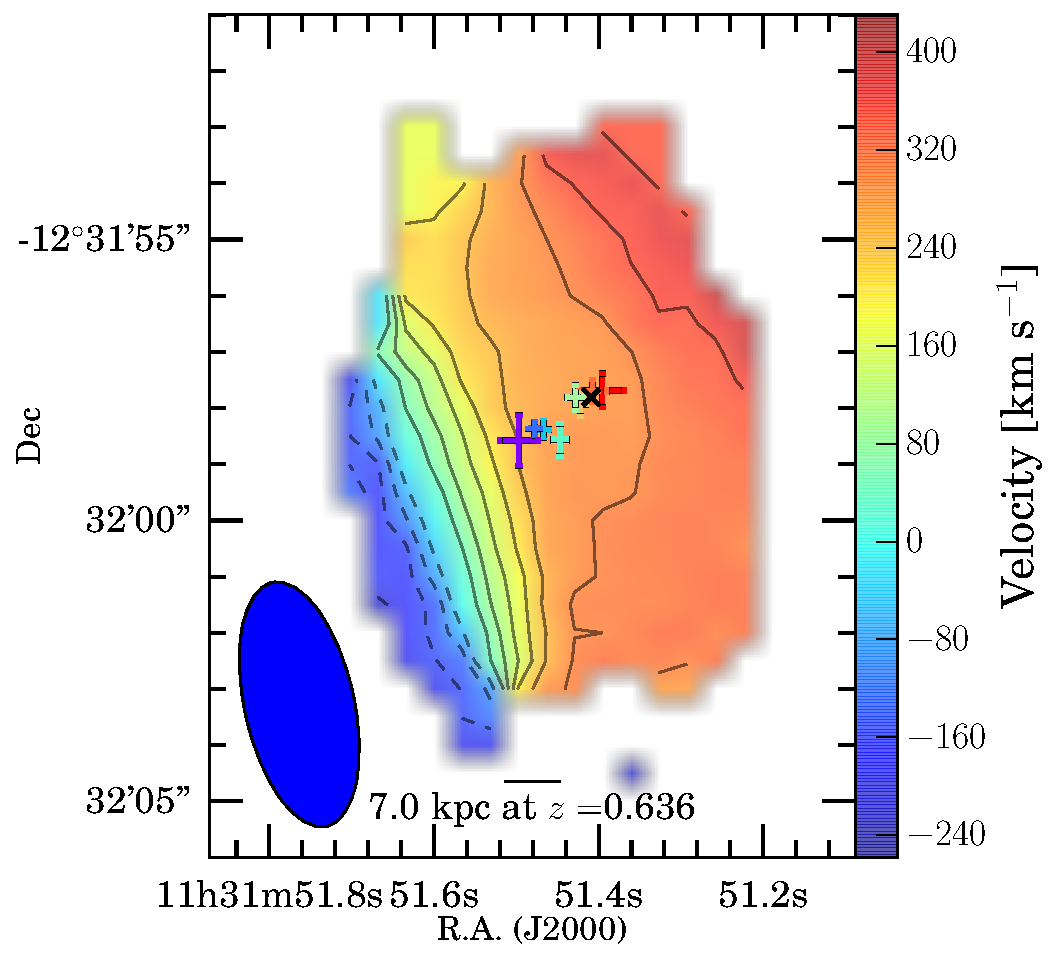
\includegraphics[trim= 0 0 0 0 clip, scale=0.43]{Figures/veloGradient_markers.pdf}
%}
%{
%\caption{\fontsize{11pt}{12.5pt}\selectfont{\textbf{Image- and source-plane velocity gradient
%of the \bco line emission in the AGN host galaxy RXJ1131.}
%Source-plane positions reconstructed from the best-fit $uv$-plane lens modeling of
%our PdBI/NOEMA \bco data in the velocity-space
%are indicated as color markers atop the observed first moment map.
%At the proposed resolution, we will be able to obtain a more accurate lens model,
%enabling us to resolve the intrinsic velocity gradient at finer details, and obtain a better-constrained rotation curve and dynamical mass estimate for this \interz quasar host galaxy.
%}}
%\label{fig:velo}}
%\end{figure}


\begin{figure}[!hptb]
\centering
\includegraphics[trim= 15 340 30 0 clip, scale=0.7]{Figures/Fig2}
\caption{\fontsize{11pt}{12.5pt}\selectfont{
\textbf{Gas morphology and dynamical constraints from
lens modelling of our NOEMA \bco data.}
{\em Left:} Extended CO emission overlaid on an optical image.
{\em Middle:}
Source-plane positions of different kinematic components
have been reconstructed from our NOEMA data using
a velocity-space lens modelling approach in the $uv$-plane,
% at the current resolution of our NOEMA data.
as indicated by color markers atop the observed first moment map.
The spectrally resolved lensed emission allows us to probe dynamical structures
on spatial scales smaller the synthesis beam.
{\em Right:} Position-velocity diagram along the source-plane major axis at PA\,=\,121$^\circ$.
Dashed line shows the best-fit rotation curve.
% The vertical error bars show the channel width for
% each model and the horizontal error bars are the
% 1$\sigma$ uncertainties on the source plane positions.
Our dynamical modelling is currently limited by the poorly resolved rotation profile in the central $\pm$2\,kpc.
At the proposed resolution, we will be able to obtain more accurate lens modelling of different kinematic components, and on smaller spatial scales,
allowing us to resolve the expected steep central gradient of the rotation curve.
This will enable us to derive more reliable estimates on the rotation velocity, inclination angle, and
dynamical mass
for this \interz quasar host galaxy.
}
\label{fig:velo}}
\end{figure}
\begin{figure*}[!htbp]
\vspace{-1.15em}
\hspace{-1.95em}
\centering
\floatbox[{\capbeside\thisfloatsetup{capbesideposition={right,center},capbesidewidth=0.5\textwidth}}]{figure}
[\FBwidth]
{
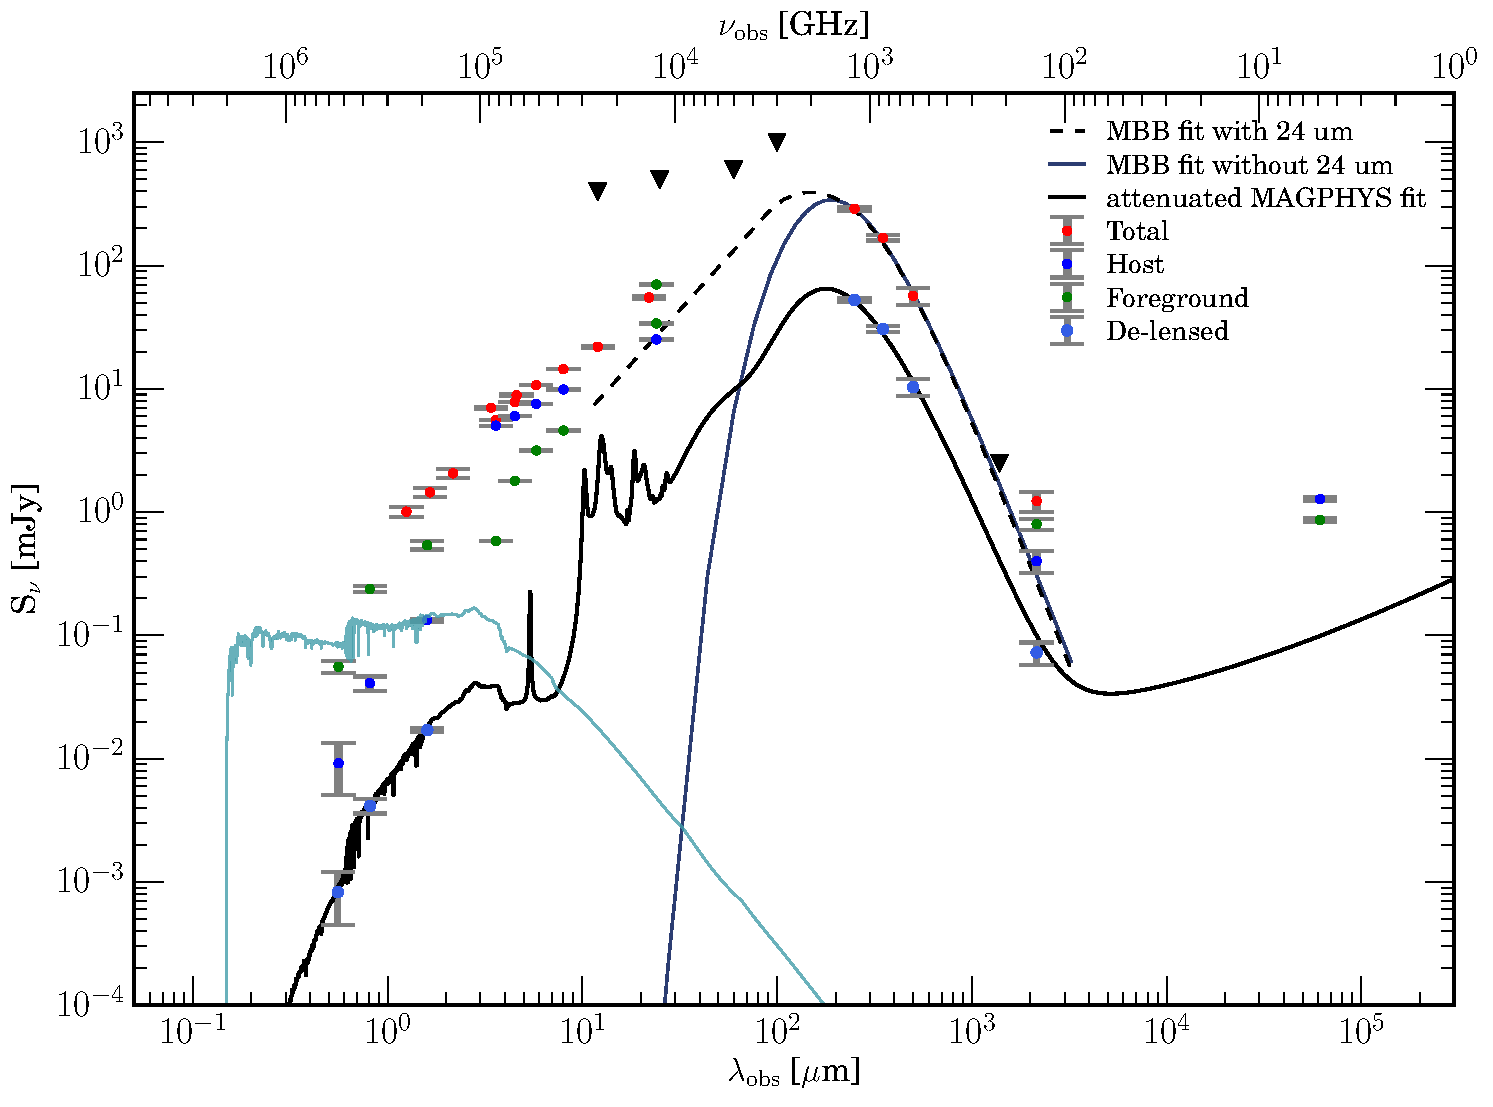
\includegraphics[trim=5 0 13 0, clip, angle=0,
width=0.50\textwidth]{Figures/FullSED_withMagphys}}
{
\hspace{-0.95em}
\caption{
% \fontsize{11pt}{12.5pt}\selectfont{
\textbf{Multi-wavelength photometry and SED models
\citep{Leung16b}.}
% }
We have de-blended rest-frame UV-to-radio
photometry in our target
(blue markers) from its foreground lensing galaxy.
The dashed and dashed-dotted lines correspond to the best-fit dust
SED models (uncorrected for lensing)
and
the black line corresponds to the best-fit full SED model (corrected for lensing).
We estimate a continuum flux of
% of $S_{\rm cont}$\ssim
$\sim$1.5$-$3.4\,mJy
by extrapolating SED models to the proposed frequency.
We thus expect to detect continuum emission underlying \cco line at $\sim$5-10$\sigma$ significance.
This will allow us to place constraints on the spatially resolved
``\SF law'' to investigate how the \SF mode of this \interz quasar host galaxy compares
to those at low and high redshift.
% }
\label{fig:SED}}}
\vspace{-0.85em}
\end{figure*}

%%%%%%%%%%%%
\noindent \textbf{References}
{\fontsize{11pt}{11pt}\selectfont
	\bibliography{RXJ_SMA}
}



\end{document}
